\section{System Overview}

We are proposing to develop the software and hardware components for a
new real time (streaming) data acquisition and data analysis system(s)
for use at the Spallation Neutron Source (SNS). The system(s) that we
propose will ultimately provide the researchers using the SNS beam
lines with effectively instant access to their reduced experimental
data both during, and after, data collection.


In order to achieve the near real-time of the scientific workflow
depicted in Figure 1, a new architecture for data acquisition and data
analysis will be developed at SNS. Whereas the previous system
architecture defined data acquisition and data analysis in isolation,
our proposed architecture will move analysis directly into the stream
of neutron events generated by the detectors and the environmental
conditions reported by the experimental environment. In this
architecture, illustrated in Figure 2, neutron data streaming from the
detectors is preprocessed and streamed to the Stream Management
Service (SMS). Sample environment data is similarly streamed to the
SMS and is aggregated with the neutron event data. The SMS stores this
data and provides a consolidated/fault tolerant data stream to
multiple consumers. In this architecture data analysis can subscribe
to this data stream on-demand, even mid-experiment, and request live
events or can request the event stream be replayed from the beginning
of the experiment. To provide live analysis capabilities to the
experimentalist at the beam line Mantid will be modified to interact
with the SMS. Other systems such as NeXus translation servers can
similarly subscribe to SMS and run translation services in parallel
with data acquisition. This streaming translation will provide users
with their datasets within seconds of the completion of the
experiment. The NeXus data files will be created and stored directly
on a high-performance parallel file system thereby allowing scalable
parallel data analysis tasks to utilize the analysis clusters at SNS
without staging data to/from high-performance storage. 



While real time data analysis of the SMS data stream will provide
users with much needed timely feedback and the ability to make
informed decisions on steering subsequent experiments, a number of
challenges must be addressed for the Mantid software to carry out
analysis of datasets in the 10-100’s of gigabytes or more. These
datasets are currently processed in Mantid using big-memory analysis
nodes (128-256 GB RAM) on which Mantid currently provides node-level
parallelism through the use of OpenMP.

\begin{figure}[h!]
  \caption{Streaming Data Analysis and Acquisition Infrastructure}
  \centering
  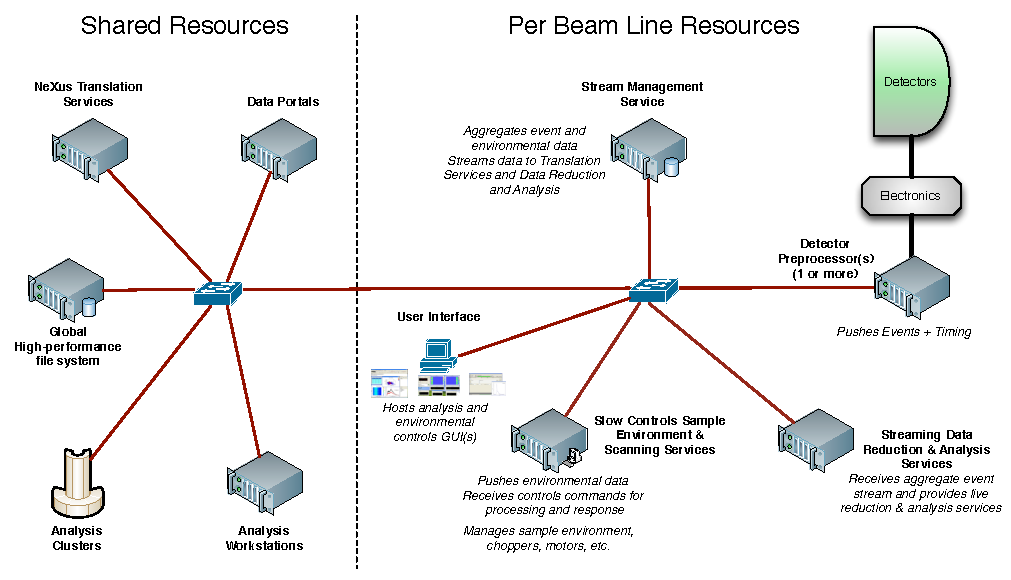
\includegraphics{workflow-high-level}
\end{figure}


As dataset sizes continue to increase, the memory requirements alone
will require parallel analysis techniques. In addition to a large
memory footprint, many analysis workloads currently require staging
datasets from one file system to another, prior to parallel data
analysis, in such an environment, the time for this staging will
dominate the analysis workflow. Moving to a parallel file system [1]
for storage within the data center will alleviate these
bottlenecks. For example, recent proto-typing of a parallel analysis
workload, showed staging of data required over 4 hours while data
reduction required only 4 minutes. Eliminating unnecessary
data-staging and enhancing Mantid with distributed memory parallelism
we will provide a near instant turn-around on common post-processing
data workloads.


Building upon this infrastructure, we will deliver an integrated
environment of experimental control and data analysis to the
end-user. Figure 3 depicts this architecture in which the end-user
interacts with the data analysis and experimental control and planning
environment through a single workstation. In addition to streaming
data analysis the experimentalist often needs to conduct
inter-comparison with previous datasets to effectively steer the
current experiment. This will be enabled through our new architecture
in which Mantid, running on the experimental workstation, can access
previous datasets through a high-performance parallel
file-system. Analysis tasks that are heavily compute or memory
footprint bound will be accelerated by developing parallel analysis
capabilities within Mantid. In this architecture, Mantid analysis
tasks can be run concurrently on an analysis cluster and the local
experimental workstation with summary analysis results displayed on
the experimenter’s workstation. 


\begin{figure}[h!]
  \caption{Combining experimental control, streaming analysis, and parallel analysis of previous runs for analysis-based experimental steering}
  \centering
  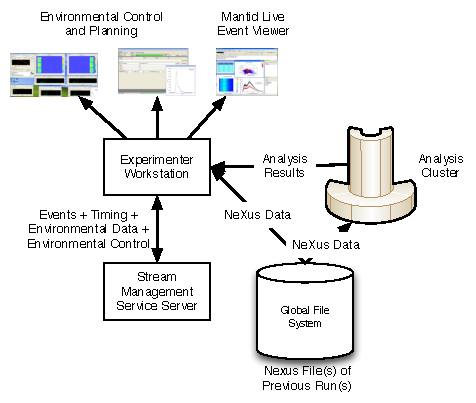
\includegraphics{workflow-high-level-workstation}
\end{figure}

